\tikzstyle{main} = [rectangle, rounded corners, 
minimum width=3cm, 
minimum height=1cm,
text centered, 
text width=3cm,
draw=black, 
fill=red!30]

\tikzstyle{output} = [rectangle, rounded corners, 
minimum width=3cm, 
minimum height=1cm,
text centered, 
text width=3cm,
draw=black, 
fill=red!50]

\tikzstyle{pale} = [rectangle, rounded corners, 
minimum width=3cm, 
minimum height=1cm,
text centered, 
text width=3cm,
draw=black, 
fill=red!10]

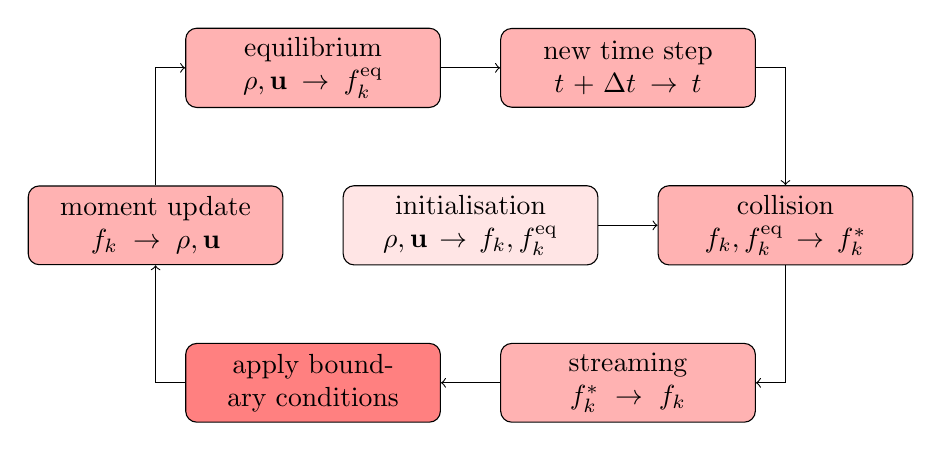
\begin{tikzpicture}[node distance=2cm]
% \node (moment) [main] {moment update
% $f_k \rightarrow \rho,\mathbf{u}$};
% \node (eqbm) [main, right of=moment, xshift=2cm] {equilibrium \par $\rho,\mathbf{u} \rightarrow f_k^{\mathrm{eq}}$};
% % \node (otpt) [pale, right of=eqbm, xshift=2cm] {output \par $\rho,\mathbf{u} \rightarrow$ disk};
% \node (stream) [main, below of=eqbm] {streaming \par $f_k^* \rightarrow f_k$};
% \node (col) [main, right of=stream] {collision \par $f_k, f_k^{\mathrm{eq}} \rightarrow f_k^*$};
% % \node (bcs) [pale, left of=stream, xshift=-2cm] {apply boundary conditions};
% \node (new time) [main, left of=stream, xshift=-2cm] {new time step \par $t + \Delta t \rightarrow t$};
% \node (force) [pale, below of=moment] {force computation};

\node (ini) [pale] {initialisation \par $\rho, \mathbf{u} \rightarrow f_k,f_k^{\mathrm{eq}}$};
\node (col) [main, right of=ini, xshift=2cm] {collision \par $f_k, f_k^{\mathrm{eq}} \rightarrow f_k^*$};
\node (stream) [main, below of=col, xshift=-2cm] {streaming \par $f_k^* \rightarrow f_k$};
\node (bcs) [output, below of=ini, xshift=-2cm] {apply boundary conditions};
\node (moment) [main, left of=ini, xshift=-2cm] {moment update \par $f_k \rightarrow \rho,\mathbf{u}$};
\node (eqbm) [main, above of=ini, xshift=-2cm] {equilibrium \par $\rho,\mathbf{u} \rightarrow f_k^{\mathrm{eq}}$};
\node (new time) [main, right of=eqbm, xshift=2cm] {new time step \par $t + \Delta t \rightarrow t$};

% \draw [->] (moment) -- (eqbm); 
% \draw [->] (eqbm) -- (otpt); 
% \draw [->] (otpt) -- (col); 
% \draw [->] (col) -- (stream); 
% % \draw [->] (stream) -- (bcs); 
% \draw [->] (stream) -- (new time); 
% \draw [->] (new time) -- (moment); 
% % \draw [->] (force) -- (moment); 

\draw [->] (ini) -- (col);
\draw [->] (col) |- (stream); 
\draw [->] (stream) -- (bcs);
\draw [->] (bcs) -| (moment);
\draw [->] (moment) |- (eqbm); 
\draw [->] (eqbm) -- (new time);
\draw [->] (new time) -| (col); 
\end{tikzpicture}
